
\documentclass[a4paper,12pt]{article}

\usepackage[utf8]{inputenc}
\usepackage[T1]{fontenc}
\usepackage[spanish]{babel}
\usepackage{tikz}
\usepackage{geometry}
\usepackage{setspace}
\usepackage{titlesec}
\usepackage{multicol}
\usepackage{fancyhdr}
\usepackage{graphicx}
\usepackage{adjustbox}
\usepackage{lastpage}
\usepackage{pgfplots}
\pgfplotsset{compat=1.18}
\usepackage{amsmath,amssymb}
\usepackage{wrapfig}
\usepackage{tabularx}
\usepackage{qrcode}
\usetikzlibrary{matrix,fit,positioning}
\usepackage{multirow}
\usepackage{colortbl}
\usepackage{hyperref}
\usepackage{booktabs}
\usepackage{array}
\usepackage{float}
\usepackage{longtable}
\usepackage{subcaption}
\usepackage{listings}
\usepackage{xcolor}
\usepackage{siunitx}
\usepackage[american]{circuitikz}

\renewcommand{\arraystretch}{1.4}
\setlength{\tabcolsep}{8pt}
\setlength{\footskip}{25pt}

\geometry{top=2.5cm,bottom=2.5cm,left=2.5cm,right=1.5cm}

\pagestyle{fancy}
\fancypagestyle{miestilo}{
    \fancyhf{}
    \fancyhead[L]{%
        \vspace{0.1cm}
        \adjustbox{valign=c,scale=0.15}{%
            \begin{tikzpicture}
                \clip (-3,-2.8) rectangle (3,2.8);
                \draw[black,line width=0.8cm] (-2.3,0)--(2.3,0);
                \draw[black,line width=0.8cm] (0,-2.85)--(0,2.85);
                \draw[black,line width=0.87cm] (0,2.8) circle(2);
                \draw[black,line width=0.87cm] (0,-2.8) circle(2);
            \end{tikzpicture}
        }%
    }
    \fancyhead[C]{\textbf{Electrónica Aplicada I}}
    \fancyhead[R]{TP N$^\circ$3 \\ 2026}
    \renewcommand{\headrulewidth}{0.4pt}
    \renewcommand{\footrulewidth}{0.4pt}
    \fancyfoot[R]{Página \thepage\ de \pageref{LastPage}}
}

\newcommand{\placeholder}[2][5cm]{%
\begin{figure}[H]
\centering
\fbox{\parbox[c][#1][c]{0.85\textwidth}{\centering #2}}
\end{figure}
}

\begin{document}

% -------------------------------------------------
% PORTADA
% -------------------------------------------------
\pagestyle{empty}
\begin{center}
    \textbf{\LARGE UNIVERSIDAD TECNOLÓGICA NACIONAL}\\[0.2cm]
    \textbf{\Large FACULTAD REGIONAL CÓRDOBA}\\[0.5cm]
    \textbf{\large INGENIERÍA ELECTRÓNICA}\\[1.5cm]

    \begin{tikzpicture}
        \clip (-3,-2.8) rectangle (3,2.8);
        \draw[black,line width=0.8cm] (-2.3,0)--(2.3,0);
        \draw[black,line width=0.8cm] (0,-2.85)--(0,2.85);
        \draw[black,line width=0.87cm] (0,2.8) circle(2);
        \draw[black,line width=0.87cm] (0,-2.8) circle(2);
    \end{tikzpicture}

    \vspace{1cm}
    \textbf{\huge Electrónica Aplicada I}\\[0.5cm]
    \rule{\textwidth}{0.4pt}\\[0.3cm]
    \textbf{\Huge Trabajo Práctico N$^\circ$3}\\[0.3cm]
    {\Large Transistor BJT en Emisor Común}\\[0.3cm]
    \rule{\textwidth}{0.4pt}\\[1.5cm]
\end{center}

\begin{flushleft}
\begin{tabular}{@{}ll}
    DOCENTE & :  Ing. Guillermo Gastón Riva\\
    & \ \ Ing. Pablo Gabriel Miklosa\\[0.2cm]
    CÁTEDRA & : Electrónica Aplicada I\\[0.2cm]
    CURSO   & : 3R4\\[0.2cm]
    ALUMNO  & :
    \begin{tabular}[t]{@{}ll}
        Gonza Elías Noel Imanol & 87669\\
        Franceschi Tobias       & 413574\\
        Pappalardo Santiago     & 94606\\
        Moyano Fabricio         & 89997\\
    \end{tabular}
\end{tabular}
\end{flushleft}

\vfill
\begin{center}
    \textbf{CÓRDOBA, ARGENTINA}\\
    \textbf{2026}
\end{center}

\newpage
\pagenumbering{arabic}
\pagestyle{miestilo}

\tableofcontents
\newpage

% -------------------------------------------------
\section{Introducción}
% -------------------------------------------------

El presente trabajo práctico tiene como objetivo diseñar, simular e implementar un amplificador
BJT en configuración de emisor común, polarizado mediante divisor resistivo y ajustado para obtener
máxima excursión simétrica (MES) de la señal de salida.

Además del análisis en corriente continua, se estudian las rectas de carga de corriente continua y
corriente alterna. Finalmente, mediante el modelo híbrido de pequeña señal, se determinan
analíticamente la impedancia de entrada $Z_i$, la impedancia de salida $Z_o$, la ganancia de
corriente $A_i$ y la ganancia de tensión $A_v$.

Los datos utilizados son:

\[
R_E=\SI{180}{\ohm},\qquad
R_C=\SI{1.2}{\kilo\ohm},\qquad
R_L=\SI{1}{\kilo\ohm}
\]

\[
V_{CC}=\SI{12}{V},\qquad
\beta=223
\]

% -------------------------------------------------
\section{Diseño para máxima excursión simétrica}
% -------------------------------------------------

\subsection{Equivalente de Thévenin de la red de entrada}

La red de polarización de base se reemplaza por su equivalente de Thévenin:

\[
V_{BB}=V_{CC}\frac{R_1}{R_1+R_2}
\]

\[
R_B=R_1\parallel R_2
=\frac{R_1R_2}{R_1+R_2}
\]

Planteando la malla de entrada:

\[
V_{BB}-I_{BQ}R_B-V_{BEQ}-I_{CQ}R_E=0
\]

y considerando:

\[
I_{BQ}=\frac{I_{CQ}}{\beta}
\]

se obtiene:

\[
I_{CQ}
=
\frac{V_{BB}-V_{BEQ}}
{R_E+\frac{R_B}{\beta}}
\]

Según el criterio de diseño indicado por la cátedra:

\[
R_E=10\frac{R_B}{\beta}
\]

por lo que:

\[
R_B=\frac{R_E\beta}{10}
\]

Reemplazando:

\[
R_B
=
\frac{180\cdot223}{10}
=
\boxed{\SI{4014}{\ohm}}
\]

% -------------------------------------------------
\subsection{Cálculo de $I_{CQ}$ para máxima excursión simétrica}
% -------------------------------------------------

La resistencia equivalente de carga en corriente alterna es:

\[
R_{CA}=R_C\parallel R_L
\]

\[
R_{CA}
=
\frac{1200\cdot1000}{1200+1000}
=
\boxed{\SI{545.45}{\ohm}}
\]

En corriente continua:

\[
R_{CC}=R_C+R_E
\]

\[
R_{CC}=1200+180
=
\boxed{\SI{1380}{\ohm}}
\]

Para máxima excursión simétrica:

\[
I_{CQ,\mathrm{MES}}
=
\frac{V_{CC}}
{R_{CA}+R_{CC}}
\]

\[
I_{CQ,\mathrm{MES}}
=
\frac{12}
{545.45+1380}
=
\boxed{\SI{6.23}{mA}}
\]

% -------------------------------------------------
\subsection{Cálculo de $V_{CEQ}$}
% -------------------------------------------------

\[
V_{CEQ}
=
V_{CC}
-
I_{CQ}(R_C+R_E)
\]

\[
V_{CEQ}
=
12
-
(6.232\,mA)(1380\,\Omega)
\]

\[
\boxed{V_{CEQ}\approx\SI{3.40}{V}}
\]

% -------------------------------------------------
\subsection{Cálculo de $V_{BB}$}
% -------------------------------------------------

Adoptando:

\[
V_{BEQ}\approx\SI{0.7}{V}
\]

de la malla de entrada:

\[
V_{BB}
=
I_{CQ}\frac{R_B}{\beta}
+
V_{BEQ}
+
I_{CQ}R_E
\]

\[
V_{BB}
=
(6.232\,mA)\frac{4014}{223}
+
0.7
+
(6.232\,mA)(180)
\]

\[
\boxed{V_{BB}\approx\SI{1.934}{V}}
\]

% -------------------------------------------------
\subsection{Cálculo de $R_1$ y $R_2$}
% -------------------------------------------------

A partir de:

\[
R_B=\frac{R_1R_2}{R_1+R_2}
\]

y

\[
V_{BB}=V_{CC}\frac{R_1}{R_1+R_2}
\]

se obtiene:

\[
R_1
=
\frac{R_B}
{1-\frac{V_{BB}}{V_{CC}}}
\]

\[
R_1
=
\frac{4014}
{1-\frac{1.934}{12}}
\]

\[
\boxed{R_1\approx\SI{4.79}{\kilo\ohm}}
\]

Para $R_2$:

\[
R_2
=
\frac{R_B}
{\frac{V_{BB}}{V_{CC}}}
\]

\[
R_2
=
\frac{4014}
{\frac{1.934}{12}}
\]

\[
\boxed{R_2\approx\SI{24.91}{\kilo\ohm}}
\]

% -------------------------------------------------
\subsection{Corrientes del divisor con valores calculados}
% -------------------------------------------------

La tensión de base es:

\[
V_B
=
I_{CQ}R_E+V_{BEQ}
\]

\[
V_B
=
(6.232\,mA)(180\,\Omega)+0.7
=
\boxed{\SI{1.822}{V}}
\]

Por lo tanto:

\[
I_{R1}
=
\frac{V_B}{R_1}
=
\frac{1.822}{4.785\,k\Omega}
\]

\[
\boxed{I_{R1}\approx\SI{380.7}{\micro A}}
\]

\[
I_{R2}
=
\frac{V_{CC}-V_B}{R_2}
=
\frac{12-1.822}{24.906\,k\Omega}
\]

\[
\boxed{I_{R2}\approx\SI{408.7}{\micro A}}
\]

\[
I_{BQ}
=
I_{R2}-I_{R1}
\]

\[
\boxed{I_{BQ}\approx\SI{27.95}{\micro A}}
\]

Como comprobación:

\[
\frac{I_{CQ}}{\beta}
=
\frac{6.232\,mA}{223}
\approx
\SI{27.95}{\micro A}
\]

% -------------------------------------------------
\subsection{Tolerancia de diseño}
% -------------------------------------------------

Considerando una tolerancia del $\pm10\%$:

\begin{table}[H]
\centering
\caption{Intervalos de tolerancia para los parámetros principales.}
\begin{tabular}{lccc}
\toprule
Parámetro & $-10\%$ & Calculado & $+10\%$\\
\midrule
$V_{BB}$ [V] & 1.741 & 1.934 & 2.127\\
$I_{CQ}$ [mA] & 5.609 & 6.232 & 6.856\\
$V_{CEQ}$ [V] & 3.059 & 3.399 & 3.739\\
\bottomrule
\end{tabular}
\end{table}

% -------------------------------------------------
\subsection{Valores normalizados}
% -------------------------------------------------

Al llevar las resistencias a valores comerciales de la serie E12, una combinación que mantiene
los parámetros principales dentro del margen aproximado de $\pm10\%$ es:

\[
\boxed{R_1=\SI{5.6}{\kilo\ohm}}
\]

\[
\boxed{R_2=\SI{27}{\kilo\ohm}}
\]

El equivalente de Thévenin resulta:

\[
R_B
=
\frac{5600\cdot27000}{5600+27000}
=
\boxed{\SI{4638}{\ohm}}
\]

\[
V_{BB}
=
12\frac{5600}{5600+27000}
=
\boxed{\SI{2.061}{V}}
\]

La corriente de reposo con valores normalizados es:

\[
I_{CQ,\mathrm{norm}}
=
\frac{V_{BB}-V_{BEQ}}
{R_E+\frac{R_B}{\beta}}
\]

\[
I_{CQ,\mathrm{norm}}
=
\frac{2.061-0.7}
{180+\frac{4638}{223}}
\]

\[
\boxed{I_{CQ,\mathrm{norm}}\approx\SI{6.780}{mA}}
\]

El error respecto del valor de diseño es:

\[
\%\,\mathrm{error}
=
\frac{6.780-6.232}{6.232}\cdot100
\approx
8.8\%
\]

por lo que permanece dentro del margen de tolerancia del $10\%$.

% -------------------------------------------------
\subsection{Punto de reposo con valores normalizados}
% -------------------------------------------------

La tensión colector-emisor es:

\[
V_{CEQ,\mathrm{norm}}
=
V_{CC}
-
I_{CQ,\mathrm{norm}}(R_C+R_E)
\]

\[
V_{CEQ,\mathrm{norm}}
=
12
-
(6.780\,mA)(1380\,\Omega)
\]

\[
\boxed{V_{CEQ,\mathrm{norm}}\approx\SI{2.644}{V}}
\]

La tensión de base:

\[
V_B
=
(6.780\,mA)(180\,\Omega)+0.7
=
\boxed{\SI{1.920}{V}}
\]

Las corrientes del divisor son:

\[
I_{R1}
=
\frac{1.920}{5.6\,k\Omega}
=
\boxed{\SI{342.9}{\micro A}}
\]

\[
I_{R2}
=
\frac{12-1.920}{27\,k\Omega}
=
\boxed{\SI{373.3}{\micro A}}
\]

\[
I_{BQ}
=
I_{R2}-I_{R1}
=
\boxed{\SI{30.4}{\micro A}}
\]

% -------------------------------------------------
\subsection{Simulación}
% -------------------------------------------------

La simulación deberá realizarse primero con los valores calculados y luego con los valores
normalizados.

\begin{figure}[H]
	\centering
	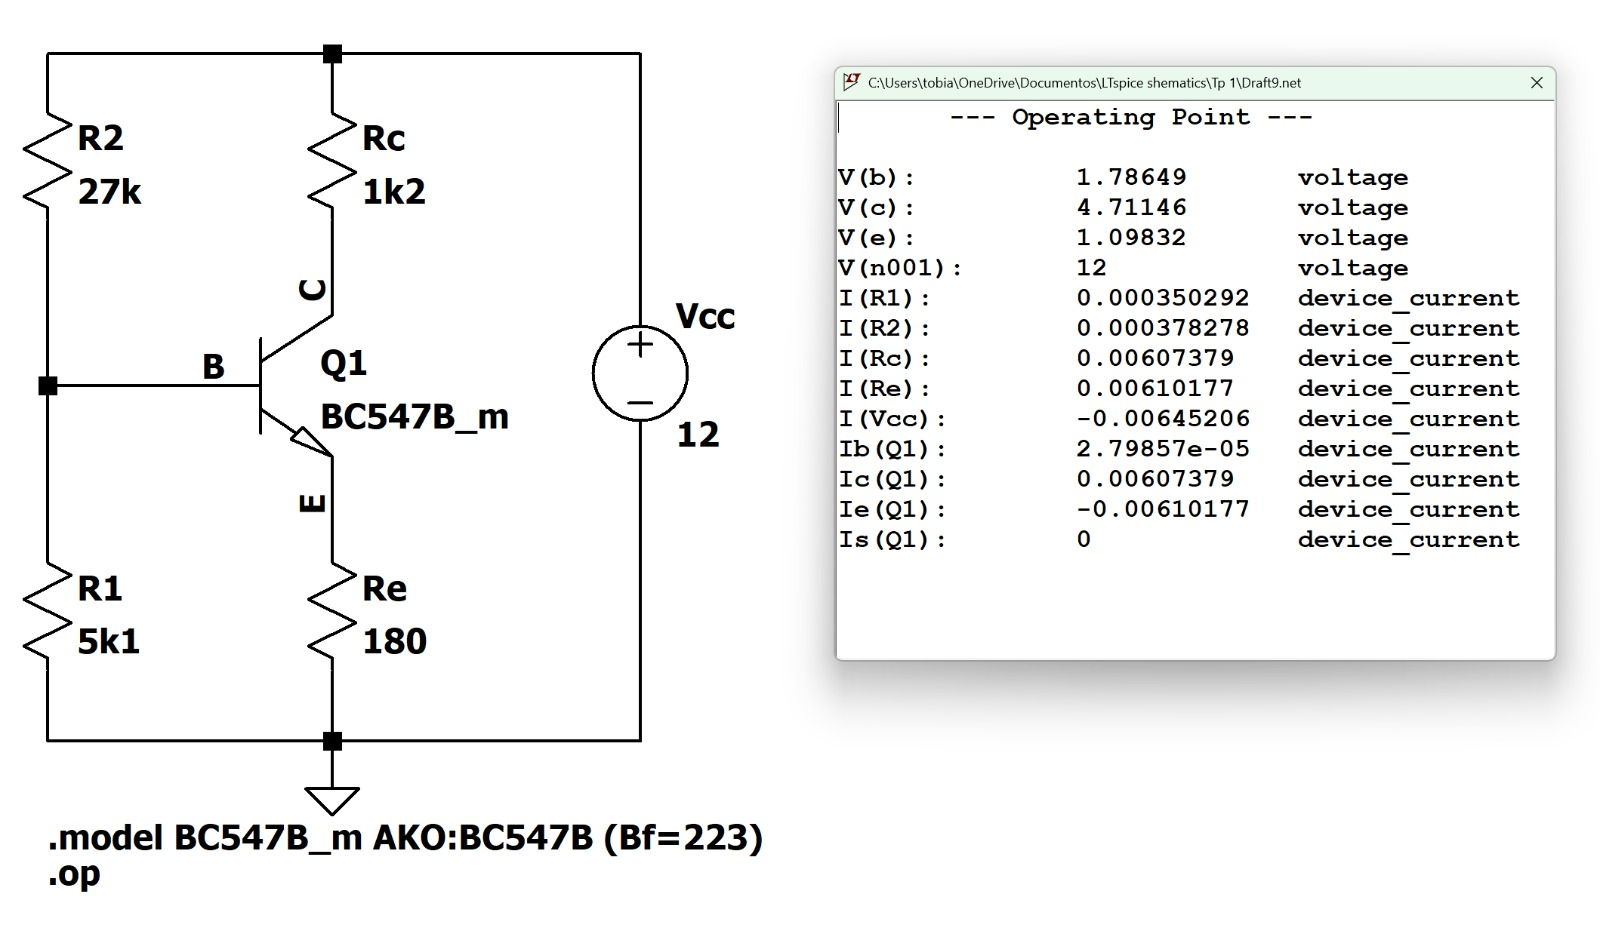
\includegraphics[width=0.95\textwidth]{simulacion1.jpeg}
	\caption{Simulación del punto de operación del amplificador en emisor común.}
	\label{fig:simulacion_punto_operacion}
\end{figure}

\begin{table}[H]
\centering
\caption{Comparación entre cálculo y simulación.}
\begin{tabular}{lccc}
\toprule
Parámetro & Calculado ideal & Normalizado teórico & Simulado\\
\midrule
$V_{BB}$ [V] & 1.934 & 2.061 & \textit{Completar}\\
$I_{CQ}$ [mA] & 6.232 & 6.780 & \textit{Completar}\\
$V_{CEQ}$ [V] & 3.399 & 2.644 & \textit{Completar}\\
$I_{BQ}$ [$\mu$A] & 27.95 & 30.4 & \textit{Completar}\\
\bottomrule
\end{tabular}
\end{table}

% -------------------------------------------------
\section{Implementación y mediciones en continua}
% -------------------------------------------------

Una vez implementado el circuito, se miden las tensiones respecto de masa y luego se calculan las
corrientes mediante ley de Ohm y ley de Kirchhoff.

\[
V_{CEQ}=V_C-V_E
\]

\[
I_{CQ}=\frac{V_{CC}-V_C}{R_C}
\]

\[
I_{R1}=\frac{V_B}{R_1}
\]

\[
I_{R2}=\frac{V_{CC}-V_B}{R_2}
\]

\[
I_{BQ}=I_{R2}-I_{R1}
\]

\begin{table}[H]
\centering
\caption{Mediciones del circuito implementado.}
\begin{tabular}{lcc}
\toprule
Parámetro & Teórico normalizado & Medido\\
\midrule
$V_{CEQ}$ & 2.644 V & \textit{Completar}\\
$I_{CQ}$ & 6.780 mA & \textit{Completar}\\
$I_{R1}$ & 342.9 $\mu$A & \textit{Completar}\\
$I_{R2}$ & 373.3 $\mu$A & \textit{Completar}\\
$I_{BQ}$ & 30.4 $\mu$A & \textit{Completar}\\
\bottomrule
\end{tabular}
\end{table}

\subsection{Implementación del circuito}


\begin{figure}[H]
	\centering
	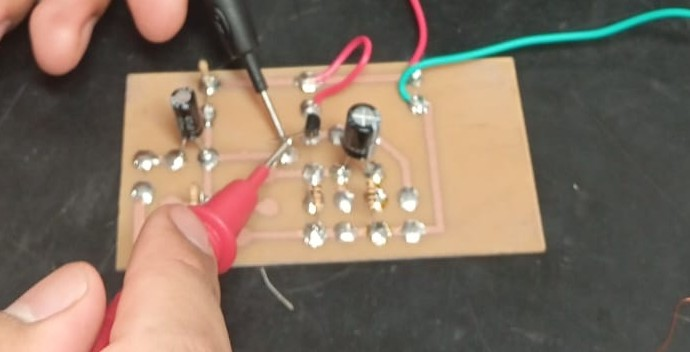
\includegraphics[width=0.7\textwidth]{circuito.jpeg}
	\caption{Implementación física del amplificador BJT en configuración de emisor común.}
	\label{fig:circuito_implementado}
\end{figure}

% -------------------------------------------------
\section{Análisis y trazado de rectas de carga}
% -------------------------------------------------

\subsection{Recta de carga de corriente continua}

La ecuación de la recta de carga de continua es:

\[
v_{CE}
=
V_{CC}
-
i_C(R_C+R_E)
\]

Para $i_C=0$:

\[
v_{CE,\max}
=
V_{CC}
=
\boxed{\SI{12}{V}}
\]

Para $v_{CE}=0$:

\[
i_{C,\max}
=
\frac{V_{CC}}{R_C+R_E}
\]

\[
i_{C,\max}
=
\frac{12}{1380}
=
\boxed{\SI{8.70}{mA}}
\]

% -------------------------------------------------
\subsection{Recta de carga de corriente alterna para el diseño MES}
% -------------------------------------------------

En alterna:

\[
R_{CA}=R_C\parallel R_L=\SI{545.45}{\ohm}
\]

La tensión aparente es:

\[
V'_{CC}
=
V_{CEQ}
+
I_{CQ}R_{CA}
\]

Para el punto de diseño MES:

\[
V'_{CC}
=
3.399
+
(6.232\,mA)(545.45\,\Omega)
\]

\[
\boxed{V'_{CC}\approx\SI{6.799}{V}}
\]

Los cortes de la recta de carga de CA son:

\[
i_C=0
\quad\Rightarrow\quad
v_{CE,\max}
=
\boxed{\SI{6.799}{V}}
\]

\[
v_{CE}=0
\quad\Rightarrow\quad
i_{C,\max}
=
\frac{6.799}{545.45}
=
\boxed{\SI{12.46}{mA}}
\]

% -------------------------------------------------
\subsection{Recta de carga de CA con valores normalizados}
% -------------------------------------------------

Utilizando el punto de reposo obtenido con $R_1=5.6\,k\Omega$ y $R_2=27\,k\Omega$:

\[
V'_{CC,\mathrm{norm}}
=
V_{CEQ,\mathrm{norm}}
+
I_{CQ,\mathrm{norm}}R_{CA}
\]

\[
V'_{CC,\mathrm{norm}}
=
2.644
+
(6.780\,mA)(545.45\,\Omega)
\]

\[
\boxed{V'_{CC,\mathrm{norm}}\approx\SI{6.342}{V}}
\]

De esta forma:

\[
i_C=0
\quad\Rightarrow\quad
v_{CE,\max}
=
\SI{6.342}{V}
\]

\[
v_{CE}=0
\quad\Rightarrow\quad
i_{C,\max}
=
\frac{6.342}{545.45}
=
\boxed{\SI{11.63}{mA}}
\]

% -------------------------------------------------
\subsection{Gráfico de las rectas de carga}
% -------------------------------------------------

\begin{figure}[H]
\centering
\begin{tikzpicture}
\begin{axis}[
    width=0.85\textwidth,
    height=0.55\textwidth,
    xlabel={$V_{CE}$ [V]},
    ylabel={$I_C$ [mA]},
    xmin=0,xmax=13,
    ymin=0,ymax=13,
    grid=both,
    legend pos=north east
]

\addplot[domain=0:12,samples=100] {(12-x)/1.38};
\addlegendentry{Recta CC}

\addplot[domain=0:6.342,samples=100] {(6.342-x)/0.54545};
\addlegendentry{Recta CA normalizada}

\addplot[only marks,mark=*] coordinates {(2.644,6.780)};
\addlegendentry{Punto Q normalizado}

\end{axis}
\end{tikzpicture}
\caption{Rectas de carga CC y CA con el punto de reposo correspondiente a los valores normalizados.}
\end{figure}

% -------------------------------------------------
\section{Análisis de pequeña señal}
% -------------------------------------------------

Para el cálculo preliminar de pequeña señal se utiliza el punto de reposo teórico obtenido con los
valores normalizados. Una vez realizadas las mediciones, puede reemplazarse $I_{CQ}$ por el valor
experimental.

\subsection{Parámetro $h_{ie}$}

Según el modelo híbrido:

\[
h_{ie}
=
h_{fe}\frac{25\,mV}{I_{CQ}}
\]

Adoptando:

\[
h_{fe}\approx\beta=223
\]

e:

\[
I_{CQ}\approx\SI{6.780}{mA}
\]

se obtiene:

\[
h_{ie}
=
223
\frac{25\,mV}{6.780\,mA}
\]

\[
\boxed{h_{ie}\approx\SI{822}{\ohm}}
\]

% -------------------------------------------------
\subsection{Impedancia de entrada}
% -------------------------------------------------

\[
Z_i
=
R_B\parallel h_{ie}
\]

\[
Z_i
=
\frac{4638\cdot822}{4638+822}
\]

\[
\boxed{Z_i\approx\SI{698}{\ohm}}
\]

% -------------------------------------------------
\subsection{Impedancia de salida}
% -------------------------------------------------

Despreciando el efecto de $h_{oe}$:

\[
\boxed{Z_o\approx R_C=\SI{1.2}{\kilo\ohm}}
\]

% -------------------------------------------------
\subsection{Ganancia de corriente}
% -------------------------------------------------

\[
A_i
=
-h_{fe}
\left(
\frac{R_C}{R_C+R_L}
\right)
\left(
\frac{R_B}{R_B+h_{ie}}
\right)
\]

\[
A_i
=
-223
\left(
\frac{1200}{1200+1000}
\right)
\left(
\frac{4638}{4638+822}
\right)
\]

\[
\boxed{A_i\approx-103.3}
\]

% -------------------------------------------------
\subsection{Ganancia de tensión}
% -------------------------------------------------

\[
A_v
=
A_i\frac{R_L}{Z_i}
\]

\[
A_v
=
-103.3
\frac{1000}{698}
\]

\[
\boxed{A_v\approx-147.9}
\]

El signo negativo representa la inversión de fase de aproximadamente $180^\circ$ propia de la
configuración de emisor común.

% -------------------------------------------------
\section{Mediciones experimentales de pequeña señal}
% -------------------------------------------------

\subsection{Impedancia de entrada $Z_i$}

A \SI{1}{kHz}, colocando una resistencia sensora $R_S$ en serie con la entrada:

\[
i_i
=
\frac{V_S-V_i}{R_S}
\]

\[
Z_i
=
\frac{V_i}{i_i}
=
R_S\frac{V_i}{V_S-V_i}
\]

\begin{table}[H]
\centering
\caption{Medición experimental de $Z_i$.}
\begin{tabular}{lc}
\toprule
Magnitud & Valor\\
\midrule
$R_S$ & \textit{Completar}\\
$V_S$ & \textit{Completar}\\
$V_i$ & \textit{Completar}\\
$Z_i$ & \textit{Calcular}\\
\bottomrule
\end{tabular}
\end{table}

% -------------------------------------------------
\subsection{Ganancia de tensión $A_v$}
% -------------------------------------------------

\[
A_v
=
\frac{V_L}{V_i}
\]

\begin{table}[H]
\centering
\caption{Medición experimental de $A_v$.}
\begin{tabular}{lc}
\toprule
Magnitud & Valor\\
\midrule
$V_L$ & \textit{Completar}\\
$V_i$ & \textit{Completar}\\
$A_v$ & \textit{Calcular}\\
\bottomrule
\end{tabular}
\end{table}

% -------------------------------------------------
\subsection{Ganancia de corriente $A_i$}
% -------------------------------------------------

\[
A_i
=
\frac{i_L}{i_i}
=
\frac{\frac{V_L}{R_L}}
{\frac{V_S-V_i}{R_S}}
\]

\begin{table}[H]
\centering
\caption{Medición experimental de $A_i$.}
\begin{tabular}{lc}
\toprule
Magnitud & Valor\\
\midrule
$V_L$ & \textit{Completar}\\
$V_S$ & \textit{Completar}\\
$V_i$ & \textit{Completar}\\
$R_S$ & \textit{Completar}\\
$A_i$ & \textit{Calcular}\\
\bottomrule
\end{tabular}
\end{table}

% -------------------------------------------------
\subsection{Impedancia de salida $Z_o$}
% -------------------------------------------------

Pasivando la entrada y aplicando la señal a la salida mediante la resistencia sensora:

\[
i_o
=
\frac{V_S-V_o}{R_S}
\]

\[
Z_o
=
\frac{V_o}{i_o}
=
R_S\frac{V_o}{V_S-V_o}
\]

\begin{table}[H]
\centering
\caption{Medición experimental de $Z_o$.}
\begin{tabular}{lc}
\toprule
Magnitud & Valor\\
\midrule
$R_S$ & \textit{Completar}\\
$V_S$ & \textit{Completar}\\
$V_o$ & \textit{Completar}\\
$Z_o$ & \textit{Calcular}\\
\bottomrule
\end{tabular}
\end{table}

% -------------------------------------------------
\section{Efecto del capacitor de desacoplo}
% -------------------------------------------------

Si se utiliza:

\[
C_E=\SI{47}{\micro F}
\]

a una frecuencia de:

\[
f=\SI{1}{kHz}
\]

su reactancia vale:

\[
X_{C_E}
=
\frac{1}{2\pi f C_E}
\]

\[
X_{C_E}
=
\frac{1}{2\pi(1000)(47\,\mu F)}
\approx
\boxed{\SI{3.39}{\ohm}}
\]

Siguiendo el análisis utilizado en el informe de referencia, la impedancia vista desde la base puede
aproximarse por:

\[
h_{ie,\mathrm{real}}
=
h_{ie}
+
(h_{fe}+1)X_{C_E}
\]

\[
h_{ie,\mathrm{real}}
=
822
+
(224)(3.39)
\]

\[
\boxed{h_{ie,\mathrm{real}}\approx\SI{1581}{\ohm}}
\]

Entonces:

\[
Z_{i,\mathrm{real}}
=
R_B\parallel h_{ie,\mathrm{real}}
\]

\[
Z_{i,\mathrm{real}}
=
\frac{4638\cdot1581}{4638+1581}
\]

\[
\boxed{Z_{i,\mathrm{real}}\approx\SI{1179}{\ohm}}
\]

Este valor deberá compararse con la medición experimental para evaluar la influencia real del
capacitor de desacoplo.

% -------------------------------------------------
\section{Conclusiones}
% -------------------------------------------------

Con $\beta=223$ y $V_{CC}=\SI{12}{V}$, el diseño ideal para máxima excursión simétrica conduce a
una corriente de reposo de aproximadamente \SI{6.23}{mA} y una tensión colector-emisor de
aproximadamente \SI{3.40}{V}.

Las resistencias calculadas para el divisor de polarización son aproximadamente:

\[
R_1=\SI{4.79}{\kilo\ohm}
\qquad\text{y}\qquad
R_2=\SI{24.91}{\kilo\ohm}.
\]

Al adoptar los valores normalizados $R_1=\SI{5.6}{\kilo\ohm}$ y
$R_2=\SI{27}{\kilo\ohm}$, la corriente de reposo calculada resulta aproximadamente
\SI{6.78}{mA}, lo que representa una diferencia cercana al $8.8\%$ respecto del diseño ideal y se
mantiene dentro de la tolerancia de diseño indicada.

Las conclusiones finales deberán completarse comparando estos resultados con la simulación y las
mediciones reales obtenidas durante el laboratorio.

% -------------------------------------------------
\section{Mediciones complementarias}
% -------------------------------------------------

\subsection{Medición de la ganancia de corriente $\beta$ del transistor}

\[
\boxed{\beta \approx h_{FE}=223}
\]

\begin{figure}[H]
	\centering
	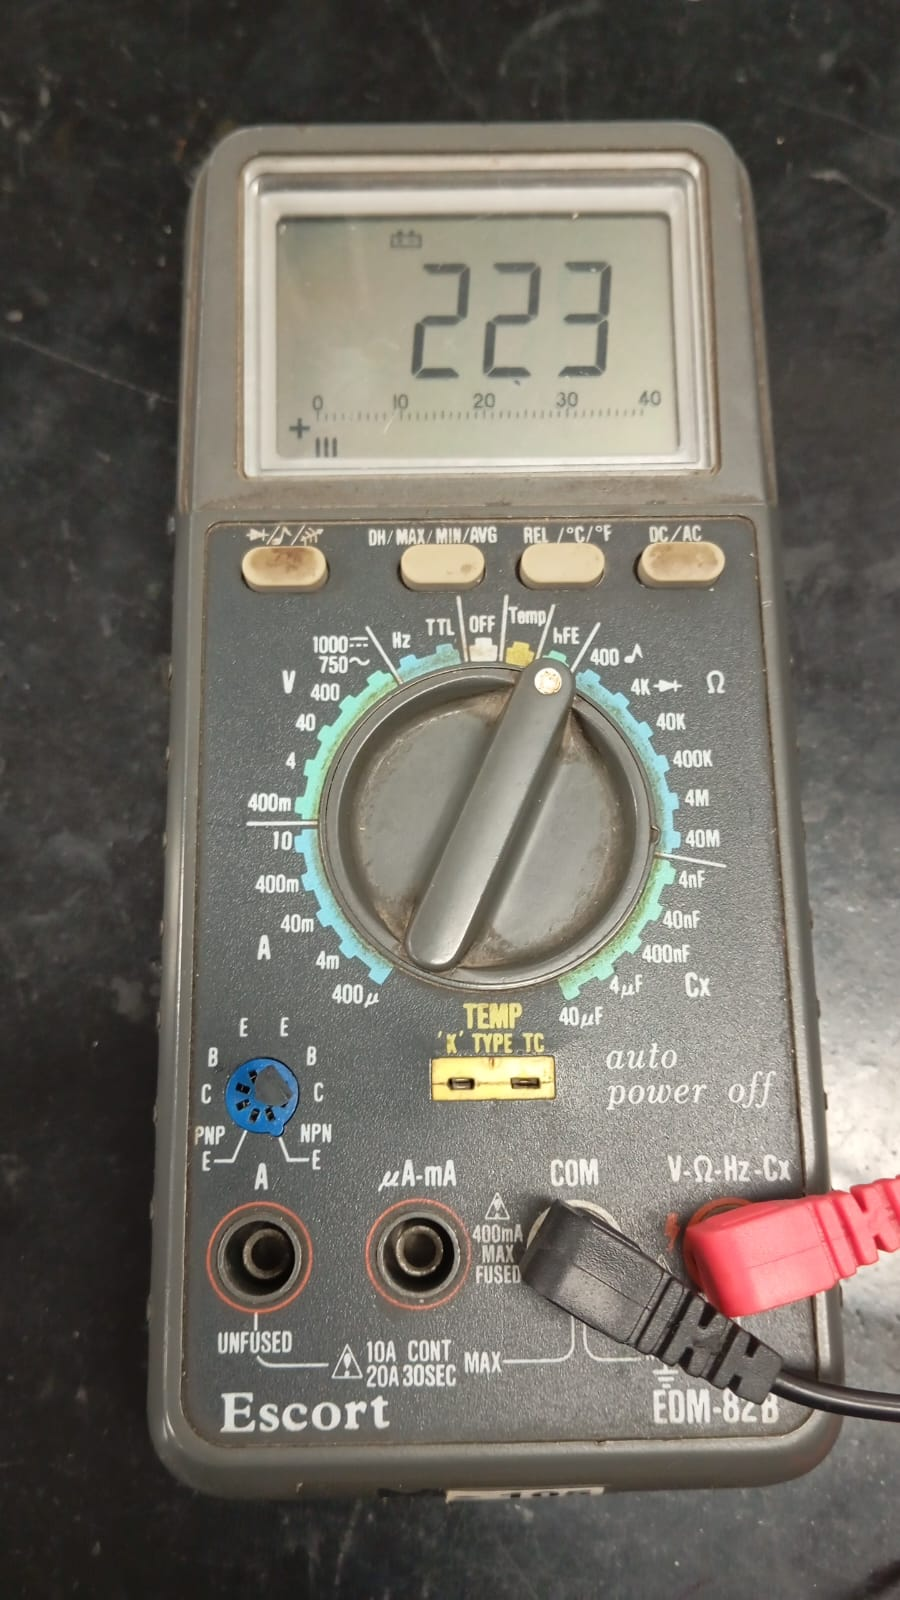
\includegraphics[width=0.3\textwidth]{beta.jpeg}
	\caption{Medición de la ganancia de corriente $h_{FE}$ del transistor utilizado.}
	\label{fig:medicion_beta}
\end{figure}







% -------------------------------------------------
\section{Bibliografía y fuentes}
% -------------------------------------------------

\begin{itemize}
    
    \item Presentación TP N$^\circ$3: Emisor Común, Electrónica Aplicada I, UTN FRC.
    \item Datasheet del transistor utilizado.
\end{itemize}

\end{document}
